\chapter{}
\label{lecture18}
\section{Функции Бесселя.}
\label{lecture18section1}
На предыдущей лекции мы имели дело с уравнением 
\begin{equation}\label{l18:eq:ast}
	-\der{}{r}\big(r\cdot f'\big)+\frac{n^2}{r}\cdot f=\lambda\cdot r\cdot f\tag{$\ast$}
\end{equation}
при граничных условиях 
\begin{equation}\label{l18:eq:ast2}
	 f(R)=0\quad\text{или}\quad\left.\pder{f}{r}\right|_{r=R}=0.\tag{$\ast\ast$}
\end{equation}
В этом уравнении $\lambda$ --- собственное значение оператора $-\Delta$. В <<Лекциях по вариационному исчислению>>~\cite{VI} мы выясняли, что при условии $f(R)=0$ --- все собственные значения $\lambda>0$, а при условии $\displaystyle\left.\pder{f}{r}\right|_{r=R}=0$ наименьшее $\lambda=0$ (соответствующая собственная функция есть константа), а все остальные $\lambda>0$. Считая далее $\lambda>0$, вводим новую независимую переменную $\rho\eqdef\sqrt{\lambda}\cdot r$ и новую неизвестную функцию $g(\rho)$:
\begin{equation}\label{l18:eq:1}
	 g(\rho)=f(r)\quad\text{при}\quad\rho=\sqrt{\lambda}\cdot r.
\end{equation} 
Тогда для функции $g(\rho)$ из уравнения~\eqref{l18:eq:ast} мы получим уравнение, которое можно записать в виде
\begin{equation}\label{l18:eq:2}
	\rho^2\cdot g''+\rho\cdot g'+(\rho^2-n^2)\cdot g=0,
\end{equation}
а граничные условия~\eqref{l18:eq:ast2} запишутся так
\begin{equation}\label{l18:eq:3}
	 g(\sqrt{\lambda}\cdot R)=0
\end{equation}
или
\begin{equation}\label{l18:eq:3A}
	 g'(\sqrt{\lambda}\cdot R)=0.\tag{\theequation A}
\end{equation}
Решения уравнения~\eqref{l18:eq:2} есть функции Бесселя $n$-ого порядка первого рода $J_n(\rho)$ и второго рода --- $N_{n}(\rho)$ --- функции Неймана. Общее решение
\begin{equation*}
	 g(\rho)=C_1\cdot J_n(\rho)+C_2\cdot N_n(\rho).
\end{equation*}
Так как нас интересуют непрерывные на $[0,R]$ решения, а $|N_n(0)|=+\infty$, то
\begin{equation*}
	 g(\rho)=C_1\cdot J_n(\rho)
\end{equation*}
и поэтому граничные условия~\eqref{l18:eq:3} и~\eqref{l18:eq:3A} приводят к уравнениям
\begin{equation}\label{l18:eq:4}
	 J_n(\sqrt{\lambda}\cdot R)=0
\end{equation}
и 
\begin{equation}\label{l18:eq:4A}
	 J_n'(\sqrt{\lambda}\cdot R)=\left.\der{J_n}{\rho}\right|_{\rho=\sqrt{\lambda}\cdot R}=0.\tag{\theequation A}
\end{equation}
Обозначим через $\mu_{nk}$ и $\mu_{nk}'$, $k=1,2,\ldots$ нули функций $J_n(\rho)$ и $J_n'(\rho)$. Тогда в случае условия~\eqref{l18:eq:4} мы получаем $\sqrt{\lambda}\cdot R=\mu_{nk}$ и при~\eqref{l18:eq:4A} $\sqrt{\lambda}\cdot R=\mu_{nk}'$, то есть
\begin{equation}\label{l18:eq:5}
	\lambda=\lambda_{nk}=\left(\frac{\mu_{nk}}{R}\right)^2\quad\text{в случае~\eqref{l18:eq:4}}
\end{equation}
или
\begin{equation}\label{l18:eq:5A}
	\lambda=\lambda_{nk}=\left(\frac{\mu'_{nk}}{R}\right)^2\quad\text{в случае~\eqref{l18:eq:4A}}.\tag{\theequation A}
\end{equation}
Обозначая решения уравнения~\eqref{l18:eq:ast}, отвечающее собственному значению $\lambda_{nk}$ через $f_{nk}(r)$, мы в силу~\eqref{l18:eq:1} и~\eqref{l18:eq:5} или~\eqref{l18:eq:5A} получим
\begin{equation}\label{l18:eq:6}
	 f_{nk}(r)=J_n\left(\frac{\mu_{nk}}{R}\cdot r\right)
\end{equation}
или
\begin{equation}\label{l18:eq:6A}
	 f_{nk}(r)=J_n\left(\frac{\mu'_{nk}}{R}\cdot r\right).\tag{\theequation A}
\end{equation}
В обоих случаях функции $f_{nk}(r)$ есть собственные функции обобщённой задачи Штурма и следовательно
\begin{equation*}
	\big(f_{nk}(r),f_{nm}(r)\big)_1\eqdef\int\limits_0^R f_{nk}(r)\cdot f_{nm}(r)\cdot r\,dr=0\quad\text{при}\quad k\neq m
\end{equation*}
и любую функцию $\Phi(r)$ из $\fLr[r;{[0,R]}]$ можно по теореме Стеклова разложить в ряд по функциям $f_{nk}(r)$, $k=1,2,\ldots$ с коэффициентами $c_{nk}=\big(\Phi(r),f_{nk}(r)\big)_1\Bigm/\norm{f_{nk}}_1^2$ (см.~<<Лекции по вариационному исчислению>>~\cite{VI}). Отсюда следуют свойства функции Бесселя:

\begin{multline*}
	\int\limits_0^R J_n\left(\frac{\beta_{nk}}{R}\cdot R\right)\cdot J_n\left(\frac{\beta_{nm}}{R}\cdot r\right)\cdot r\,dr=0\quad\text{при}\quad m\neq k,\\\text{где }\begin{array}{lll}
		&\beta_{nk}=\mu_{nk},& \beta_{nm}=\mu_{nm}\\
		\text{или}&&\\
		&\beta_{nk}=\mu'_{nk},& \beta_{nm}=\mu'_{nm}.
	\end{array}
\end{multline*}
\begin{multline*}
	\Phi(r)=\sum\limits_{k=1}^{\infty} C_{nk}\cdot J_{n}\left(\frac{\beta_{nk}}{R}\cdot r\right),\\\text{ где }c_{nk}=\left.\int\limits_0^R\Phi(r)\cdot J_n\left(\frac{\beta_{nk}}{R}\cdot r\right)\cdot r\,dr\middle/\int\limits_0^R r\cdot J_n^2\left(\frac{\beta_{nk}}{R}\cdot r\right)\,dr\right.,\\ \begin{array}{ll}
		&\beta_{nk}=\mu_{nk}\\
		\text{или}&\\
		&\beta_{nk}=\mu'_{nk}.
	\end{array}
\end{multline*}
Эти соотношения выводились в <<Лекциях по вариационному исчислению>>~\cite{VI}, но  здесь уместно было их повторить$\dots$

Возвращаемся к уравнению Бесселя~\eqref{l18:eq:2}. Отыскивая его решение в виде рядов, получим
\begin{equation}\label{l18:eq:7}
	 J_n(\rho)=\left(\frac{\rho}{2}\right)^n\cdot\sum\limits_{p=0}^{\infty}(-1)^p\cdot\frac{1}{p!\cdot(p+n)!}\cdot\left(\frac{\rho}{2}\right)^{2\cdot p},
\end{equation}
где $0!=1$ по определению,
\begin{equation*}
	 N_n(\rho)=c\cdot\ln\rho\cdot J_n(\rho)+\rho^{-n}\cdot\sum\limits_{k=0}^{\infty}d_k\cdot\rho^{k},\quad d_0\neq0.
\end{equation*}
Мы видим, что $J_n(0)=0$ при $n\neq0$, $J_n(\rho)\in\Cfn[{[0,R]}]{2}$.	Функция Неймана $N_n(\rho)$ при $\rho=0$ обращается в бесконечность при $n=0$ за счёт $\ln\rho$, при $n>0$ за счёт $\rho^{-n}$.

До сих пор здесь мы рассматривали функции Бесселя целого порядка $n$, хотя в курсе вариационного исчисления мы имели дело и с функциями произвольного порядка $\nu$. \emph{Выясним аналитический вид функций $J_{\nu}(\rho)$ и $N_{\nu}(\rho)$ при не целых $\nu$ и при отрицательных значениях $\nu$.} Эти функции являются решениями уравнения 
\begin{equation}\label{l18:eq:8}
	\rho^2\cdot f''+\rho\cdot f'+(\rho^2-\nu^2)\cdot f=0.
\end{equation} 
Для их определения нам понадобится \emph{Гамма-функция}:
\begin{equation}\label{l18:eq:9}
	\Gamma(\beta)\eqdef\int\limits_{0}^{\infty}x^{\beta-1}\cdot e^{-x}\,dx.
\end{equation}
При $\Re\beta>0$ интеграл для $\Gamma(\beta)$ сходится. Продолжим аналитическую при $\Re\beta>0$ функцию $\Gamma(\beta)$ на всю комплексную плоскость $\beta$, $\beta\?=\beta_1+i\cdot\beta_2$. Делаем это шагами. Предположим, что $\Re\beta>1$, тогда мы можем провести интегрирование по частям в~\eqref{l18:eq:9}:
\begin{multline}\label{l18:eq:10}
	\Gamma(\beta)=\int\limits_{0}^{\infty}\underbrace{x^{\beta-1}}_{u}\cdot \underbrace{e^{-x}\,dx}_{dv}=-x^{\beta-1}\cdot e^{-x}\mathop{\Big|}\limits_{0}^{\infty}+(\beta-1)\cdot\int\limits_{0}^{\infty}x^{\beta-2}\cdot e^{-x}\,dx=\\=(\beta-1)\cdot\Gamma(\beta-1).
\end{multline}
Правая часть~\eqref{l18:eq:10} определена в полуплоскости $\Re\beta>1$, а левая часть~--- при $\Re\beta>0$. Из~\eqref{l18:eq:10}
\begin{equation}\label{l18:eq:11}
	\Gamma(\beta-1)=\frac{\Gamma(\beta)}{\beta-1}.
\end{equation}
Будем считать правую часть~\eqref{l18:eq:11} продолжением функции $\Gamma(\beta-1)$ на область $\Re\beta>0$, в которой определена функция $\Gamma(\beta)$. Но тогда в левой части~\eqref{l18:eq:11} аргумент $\beta-1$ у функции $\Gamma(\beta-1)$ имеет $\Re(\beta-1)>-1$. Таким образом, Гамма-функция определена при аргументе расположенном справа от прямой $\Re\beta=-1$. Но тогда правая часть~\eqref{l18:eq:11} определена при $\Re\beta>-1$. Значит левая при $\Re(\beta-1)>-2$ ибо $\Re\beta>-1$ и так далее. Таким образом мы продолжим Гамма-функцию на всю комплексную плоскость. При таком продолжении, однако, при $\Re\beta=0,\,-1,\,-2\,\ldots$ $|\Gamma(\beta)|=+\infty$. 

Отыскивая решение в виде ряда по степеням $\rho$, мы получим два решения уравнения~\eqref{l18:eq:8}:
\begin{equation*}
	\begin{array}{rcl}  J_{\nu}(\rho)&=&\displaystyle\left(\frac{\rho}{2}\right)^{\nu}\cdot\sum\limits_{s=0}^{\infty}\dfrac{(-1)^s\cdot\left(\frac{\rho}{2}\right)^{2\cdot s}}{\Gamma(s+1)\cdot\Gamma(\nu+s+1)},\\[12pt]  J_{-\nu}(\rho)&=&\displaystyle\left(\frac{\rho}{2}\right)^{-\nu}\cdot\sum\limits_{s=0}^{\infty}\dfrac{(-1)^s\cdot\left(\frac{\rho}{2}\right)^{2\cdot s}}{\Gamma(s+1)\cdot\Gamma(-\nu+s+1)}.
	\end{array}
\end{equation*} 
Если $\nu$ --- не целое, то $J_{\nu}(\rho)$ и $J_{-\nu}(\rho)$ --- линейно независимы, ибо при $\nu>0$ $J_{\nu}(\rho)$ --- аналитическая функция без особенностей, а $J_{-\nu}(\rho)$ имеет полюс при $\rho=0$. Поэтому общее решение~\eqref{l18:eq:8} есть
\begin{equation*}
	 c_1\cdot J_{\nu}(\rho)+c_2\cdot J_{-\nu}(\rho).
\end{equation*} 
При $\nu$ --- целом 
\begin{equation}\label{l18:eq:12}
	 J_{-n}(\rho)=(-1)^{n}\cdot J_n(\rho).
\end{equation}

\noindent\textbf{Задание. }Проверить соотношение~\eqref{l18:eq:12} (подсказка: использовать то, что $|\Gamma(\nu)|=\infty$ при $\nu=0,\,-1,\,-2,\ldots$)
\vspace*{0.2cm}

\noindent В силу~\eqref{l18:eq:12} функция $J_{-n}(\rho)$ не является вторым линейно независимым решением уравнения~\eqref{l18:eq:8}, поэтому в качестве второго решения, которое вместе с $J_{\nu}(\rho)$ образует базис в пространстве решений~\eqref{l18:eq:8}, берут функцию Неймана
\begin{equation*}
	 N_{\nu}(\rho)=\dfrac{J_{\nu}(\rho)\cdot\cos\left(\nu\cdot\pi\right)-J_{-\nu}(\rho)}{\sin\left(\nu\cdot\pi\right)}.
\end{equation*}
То, что при $\nu$ --- не целом функции $J_{\nu}(\rho)$ и $N_{\nu}(\rho)$ линейно независимы~--- очевидно, а при $\nu\to n$ надо раскрывать неопределённость типа $\frac{0}{0}$.

Наряду с функциями Бесселя и Неймана в приложениях часто встречаются функции Ханкеля (Hankel) первого и второго рода:
\begin{equation*}
	 H_{\nu}^{1(2)}\eqdef J_{\nu}(\rho)\pm i\cdot N_{\nu}(\rho).
\end{equation*}

Функции Бесселя, Неймана и Ханкеля хорошо изучены и существует огромное количество разнообразных формул для них, их производных, интегралов от них и так далее. Приведу некоторые из них (в основном для ориентировки, а не для заучивания.) Асимптотика при $\rho\gg1$:
\begin{equation*}
	\begin{array}{rcl}
		J_{\nu}(\rho)&=&\displaystyle\sqrt{\frac{2}{\pi\cdot\rho}}\left[\cos\left(\rho-\frac{\nu\cdot\pi}{2}-\frac{\pi}{4}\right)+O\left(\frac{1}{\rho}\right)\right],\\[12pt]
		N_{\nu}(\rho)&=&\displaystyle\sqrt{\frac{2}{\pi\cdot\rho}}\left[\sin\left(\rho-\frac{\nu\cdot\pi}{2}-\frac{\pi}{4}\right)+O\left(\frac{1}{\rho}\right)\right].
	\end{array}
\end{equation*}
То есть главная часть асимптотики --- это замодулированные множителем $1/\sqrt{\rho}$ косинус и синус; от порядка $\nu$ функции зависит только фузовый сдвиг. Отсюда при $\rho\gg1$
\begin{equation*}
	 H_{\nu}^{1(2)}(\rho)=\displaystyle\sqrt{\frac{2}{\pi\cdot\rho}}\left[e^{\textstyle \pm i\cdot\left(\textstyle\rho-\frac{\nu\cdot\pi}{2}-\frac{\pi}{4}\right)}+O\left(\frac{1}{\rho}\right)\right].
\end{equation*} 
Далее
\begin{equation*}
	\int\limits_{0}^{R}\rho\cdot J_{n}^2\left(\frac{\mu_{nk}}{R}\cdot\rho\right)\,d\rho=\frac{R^2}{2}\cdot\left[J_n'(\mu_{nk})\right]^2,
\end{equation*}
\begin{equation}\label{l18:eq:13}
	\der{}{\rho}\left(\frac{J_{\nu}(\rho)}{\rho^{\nu}}\right)=-\frac{J_{\nu+1}(\rho)}{\rho^{\nu}};\quad\der{}{\rho}\Big(\rho^{\nu}\cdot J_{\nu}(\rho)\Big)=\rho^{\nu}\cdot J_{\nu-1}(\rho).		
\end{equation}
Используя формулы~\eqref{l18:eq:13} можно найти асимптотику для $J_{\nu}'(\rho)$.  Мы видели, что в общем случае функции Бесселя даются рядами, но в случае полуцелого аргумента функции Бесселя выражаются через элементарные функции:
\begin{gather*}
	 J_{n+\frac{1}{2}}(\rho)=\sqrt{\frac{2}{\pi\cdot\rho}}\cdot\rho^{n+1}\left(-\frac{1}{\rho}\cdot\der{}{\rho}\right)^{n+1}\cos\rho;\\ N_{n+\frac{1}{2}}(\rho)=\sqrt{\frac{2}{\pi\cdot\rho}}\cdot\rho^{n+1}\left(-\frac{1}{\rho}\cdot\der{}{\rho}\right)^{n+1}\sin\rho;\\
	 H_{n+\frac{1}{2}}^{1(2)}(\rho)=\sqrt{\frac{2}{\pi\cdot\rho}}\cdot\rho^{n+1}\left(-\frac{1}{\rho}\cdot\der{}{\rho}\right)^{n+1}e^{\pm i\cdot\rho}.
\end{gather*}
\section{Модифицированные функции Бесселя.}
\label{lecture18section2}
Уравнение Бесселя~\eqref{l18:eq:8} формально верно для любых $\rho$. Положим там $i\cdot\rho$ вместо $\rho$ и пусть $f(\rho)\equiv g(i\cdot\rho)$, тогда
\begin{equation*}
	 (i\cdot\rho)^2\cdot\dder{f}{(i\cdot\rho)}+i\cdot\rho\cdot\der{f}{(i\cdot\rho)}+\big[(i\cdot\rho)^2-\nu^2\big]\cdot f=0,
\end{equation*}
то есть
\begin{equation}\label{l18:eq:14}
	 \rho^2\cdot f''+\rho\cdot f'-(\rho^2+\nu^2)\cdot f=0.
\end{equation}
Это уравнение для модифицированных функций Бесселя $\nu$-ого порядка, которые обозначаются через $I_{\nu}(\rho)$. По построению 
\begin{equation*}
	 I_{\nu}(\rho)=J_{\nu}(i\cdot\rho)
\end{equation*}
поэтому 
\begin{multline}\label{l18:eq:15}
	I_{\nu}(\rho)=\left(\frac{i\cdot \rho}{2}\right)^{\nu}\cdot\sum\limits_{s=0}^{\infty}(-1)^s\cdot\dfrac{\left(\frac{i\cdot\rho}{2}\right)^{2\cdot s}}{\Gamma(s+1)\cdot\Gamma(-\nu+s+1)}=\\=e^{\textstyle i\cdot\frac{\nu}{2}\cdot\pi}\cdot\left(\frac{ \rho}{2}\right)^{\nu}\cdot\sum\limits_{s=0}^{\infty}\cdot\dfrac{\left(\frac{\rho}{2}\right)^{2\cdot s}}{\Gamma(s+1)\cdot\Gamma(-\nu+s+1)}. 
\end{multline}
Так как решение~\eqref{l18:eq:14} определено с точностью до постоянного множителя, то примем за $I_{\nu}(\rho)$ произведение 
\begin{equation*}
	 I_{\nu}(\rho)\eqdef e^{\textstyle- i\cdot\frac{\nu}{2}\cdot\pi}\cdot J_{\nu}(i\cdot\rho),
\end{equation*}
Это обеспечивает вещественность функции $I_{\nu}(\rho)$. Из~\eqref{l18:eq:15} видно, что в отличие от ряда для $J_{\nu}(\rho)$ ряд для $I_{\nu}(\rho)$ не является знакопеременным и $I_{\nu}(\rho)\to+\infty$ при $\rho\to\infty$. Далее как и для уравнения~\eqref{l18:eq:8} вторым линейно независимым решением~\eqref{l18:eq:14} является функция $I_{-\nu}(\rho)$, исключая целые значения $\nu$, для которых 
\begin{equation*}
	 I_{-n}(\rho)=I_{n}(\rho).
\end{equation*}
Поэтому в качестве второго линейно независимого решения уравнения~\eqref{l18:eq:14} берут не $I_{-\nu}(\rho)$, а функцию 
\begin{equation*}
	 K_{\nu}(\rho)=\pi\cdot\dfrac{I_{-\nu}(\rho)-I_{\nu}(\rho)}{2\cdot\sin(\nu\cdot\pi)}.
\end{equation*}
Эта функция называется функцией Макдональда\footnote{Не Макдональдса!} или функцией Бесселя $3^{\text{его}}$ рода. С модифицированными функциями Бесселя мы неоднократно встретимся в дальнейшем.
\section{Распространение тепла.}
\label{lecture18section3}
Пусть в пространстве выделен произвольный объём $V$ и $u(P,t)$ --- температура в точке $P=(x,y,z)$ в момент $t$.




\begin{figure}[H]\centering
\tikzset{every picture/.style={line width=0.75pt}} %set default line width to 0.75pt        

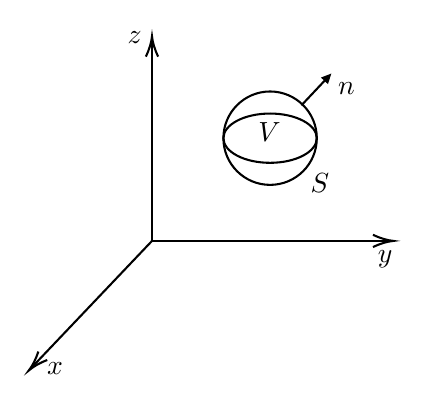
\begin{tikzpicture}[x=0.75pt,y=0.75pt,yscale=-0.9,xscale=0.9]
	%uncomment if require: \path (0,300); %set diagram left start at 0, and has height of 300
	
	%Straight Lines [id:da814828708381407] 
	\draw    (133.78,164) -- (261,164) ;
	\draw [shift={(263,164)}, rotate = 180] [color={rgb, 255:red, 0; green, 0; blue, 0 }  ][line width=0.75]    (10.93,-3.29) .. controls (6.95,-1.4) and (3.31,-0.3) .. (0,0) .. controls (3.31,0.3) and (6.95,1.4) .. (10.93,3.29)   ;
	%Straight Lines [id:da16718611697435493] 
	\draw    (133.78,164) -- (69.16,231.96) ;
	\draw [shift={(67.78,233.41)}, rotate = 313.56] [color={rgb, 255:red, 0; green, 0; blue, 0 }  ][line width=0.75]    (10.93,-3.29) .. controls (6.95,-1.4) and (3.31,-0.3) .. (0,0) .. controls (3.31,0.3) and (6.95,1.4) .. (10.93,3.29)   ;
	%Straight Lines [id:da848152640173949] 
	\draw    (133.78,164) -- (133.78,56.41) ;
	\draw [shift={(133.78,54.41)}, rotate = 450] [color={rgb, 255:red, 0; green, 0; blue, 0 }  ][line width=0.75]    (10.93,-3.29) .. controls (6.95,-1.4) and (3.31,-0.3) .. (0,0) .. controls (3.31,0.3) and (6.95,1.4) .. (10.93,3.29)   ;
	%Shape: Circle [id:dp41976582742621127] 
	\draw   (172,109) .. controls (172,95.19) and (183.19,84) .. (197,84) .. controls (210.81,84) and (222,95.19) .. (222,109) .. controls (222,122.81) and (210.81,134) .. (197,134) .. controls (183.19,134) and (172,122.81) .. (172,109) -- cycle ;
	%Shape: Ellipse [id:dp07540167273586151] 
	\draw   (172,109) .. controls (172,101.71) and (183.19,95.81) .. (197,95.81) .. controls (210.81,95.81) and (222,101.71) .. (222,109) .. controls (222,116.29) and (210.81,122.19) .. (197,122.19) .. controls (183.19,122.19) and (172,116.29) .. (172,109) -- cycle ;
	%Straight Lines [id:da21839824584502154] 
	\draw    (213.78,91.41) -- (227.73,76.59) ;
	\draw [shift={(229.78,74.41)}, rotate = 493.26] [fill={rgb, 255:red, 0; green, 0; blue, 0 }  ][line width=0.08]  [draw opacity=0] (5.36,-2.57) -- (0,0) -- (5.36,2.57) -- cycle    ;
	
	% Text Node
	\draw (76,227.4) node [anchor=north west][inner sep=0.75pt]    {$x$};
	% Text Node
	\draw (253,167.4) node [anchor=north west][inner sep=0.75pt]    {$y$};
	% Text Node
	\draw (119,50.4) node [anchor=north west][inner sep=0.75pt]    {$z$};
	% Text Node
	\draw (231.78,77.81) node [anchor=north west][inner sep=0.75pt]    {$\bm{n}$};
	% Text Node
	\draw (189,99.21) node [anchor=north west][inner sep=0.75pt]    {$V$};
	% Text Node
	\draw (217,126.4) node [anchor=north west][inner sep=0.75pt]    {$S$};
	
	
\end{tikzpicture}
	\caption{~}
\label{l18:fig:1}
\end{figure}

Выведем уравнение, которому удовлетворяет функция $u(P,t)$. Вывод --- на основе уравнения теплового баланса. Рассмотрим произвольный временной интервал $[t_0,t_1]$. Пусть $Q_1$ --- тепло, выделенное за это время источниками внутри $V$, $Q_2$ --- потеря (или приток) тепла через границу $S$ объёма $V$ за время от $t_0$ до $t_1$, $Q_3$ --- запасённое тепло. Тогда 
\begin{equation}\label{l18:eq:16}
	 Q_1+Q_2=Q_3,
\end{equation}
где $Q_2>0$ если имеется приток тепла через границу, и $Q_2<0$ --- если убыль. Найдём выражения для $Q_i$.

Величина $Q_1$ определяется объёмной плотностью мощности источников, то есть теплом, выделенным в единицу времени в единичном объёме. Обозначим эту мощность через $f(P,t)$. Тогда 
\begin{equation}\label{l18:eq:17}
	 Q_1=\int\limits_{t_0}^{t_1}\iiint\limits_{V} f(P,t)\,dVdt. 
\end{equation}
Что касается $Q_2$, то ясно, что эта величина зависит от разницы температур на границы $S$, то есть от разницы внутри и вне $V$, а эта разность определяется нормальной производной $\pder{u}{n}$ на $S$. Поэтому
\begin{equation}\label{l18:eq:18}
	 Q_2=\int\limits_{t_0}^{t_1}\iint\limits_{S} k\cdot\pder{u}{n}\,dSdt, 
\end{equation}
где $k$ --- коэффициент, зависящий от теплопроводности в рассматриваемой точке $P$ в момент времени $t$. Заметим, что если $\pder{u}{n}>0$, то есть <<наружная>> температура выше <<внутренней>>, то $Q_2>0$ --- приток тепла, а если $\pder{u}{n}<0$, то внутри температура выше и, значит, будет отток тепла. Наконец, запасённое элементарной массой $\rho\cdot\Delta V$ за время $t_1-t_0$ тепло согласно школьным формулам есть
\begin{equation*}
	 \big[u(P,t_1)-u(P,t_0)\big]\cdot c\cdot\rho\cdot\Delta V,
\end{equation*} 
где $\rho$ и $c$ --- плотность и теплоёмкость вещества в $V$. Поэтому 
\begin{equation}\label{l18:eq:19}
	 Q_3=\iiint\limits_{V}\big[u(P,t_1)-u(P,t_0)\big]\cdot c\cdot\rho\,dV=\int\limits_{t_0}^{t_1}\iiint\limits_{V}\pder{u}{t}\cdot c\cdot\rho\,dVdt.
\end{equation}
Здесь мы считаем, что $c$ и $\rho$ не зависят от времени. 

Прежде чем подставлять найденные величины $Q_i$ в уравнение теплового баланса~\eqref{l18:eq:16} заметим, что в силу формулы Остроградского--Гаусса (при $k\cdot\grad u$ лежащем в $\Cfn[]{1}(V)$ и в $\Cfn[]{}(\overline{V})$)
\begin{equation*}
	 \iint\limits_{S}k\cdot\pder{u}{n}\,dS=\iiint\limits_{V}\Div(k\cdot\grad u)\,dV
\end{equation*}
и поэтому в силу~\eqref{l18:eq:18}
\begin{equation}\label{l18:eq:20}
	 Q_2=\int\limits_{t_0}^{t_1}\iiint\limits_{V}\Div(k\cdot\grad u)\,dVdt.
\end{equation}
Подставляя~\eqref{l18:eq:17},~\eqref{l18:eq:19},~\eqref{l18:eq:20} в~\eqref{l18:eq:16} и перенеся там $Q_3$ в левую часть соотношения, получим
\begin{equation}\label{l18:eq:21}
	 \int\limits_{t_0}^{t_1}\iiint\limits_{V}\left[f(P,t)+\Div(k\cdot\grad u)-\pder{u}{t}\cdot c\cdot\rho\right]\,dVdt=0.
\end{equation}
Так как интервал времени может быть любым и объём $V$ произвольный, то из~\eqref{l18:eq:21} следует, что в любой точке $P$ и в любой момент времени подынтегральное выражение равно нулю, откуда 
\begin{equation}\label{l18:eq:22}
	 c\cdot\rho\cdot\pder{u}{t}=\pder{}{x}\left(k\cdot\pder{u}{x}\right)+\pder{}{y}\left(k\cdot\pder{u}{y}\right)+\pder{}{z}\left(k\cdot\pder{u}{z}\right)+f(P,t). 
\end{equation}
Отсюда при постоянных $c$, $\rho$, $k$, поделив на $c\cdot\rho$ и положив $a^2={k}/(c\cdot\rho)$, получим
\begin{equation}\label{l18:eq:23}
	\pder{u}{t}=a^2\cdot\Delta u+\tilde{f}(P,t),
\end{equation}
где $\tilde{f}(P,t)=\dfrac{f(P,t)}{c\cdot\rho}$.

Для получения единственного решения этой задачи надо знать начальные и граничные условия. Пусть задача решается в фиксированной области $\Omega\subset\R^3$ и $S=\partial\Omega$ --- граница области. Возможные типы граничных условий.
\begin{enumerateD}
	\item На границе задан температурный режим:
	\begin{equation*}
		 u(P,t)\Big|_{S}=g(P,t).
	\end{equation*}
	Простейший случай --- поддерживается нулевая температура, то есть $g(P,t)=0$.
	
	\item На границе задан тепловой поток:
	\begin{equation*}
		 k\cdot\left.\pder{u}{n}\right|_{S}=h(P,t).
	\end{equation*}
	Простейший случай --- граница теплоизолирована: $h(P,t)=0$.
	
	\item На границе происходит излучение в окружающую среду по закону Ньютона
	\begin{equation*}
		 \pder{u}{n}+\sigma\cdot(u-u_0)\Big|_{S}=0,
	\end{equation*}
	где $u_0(P,t)$ --- температура окружающей среды, $\sigma>0$ --- постоянный коэффициент.
\end{enumerateD} 
Разумеется на разных участках поверхности $S$ могут быть свои на каждом участке граничные условия.

Теперь о начальных условиях. В задачах о колебаниях струны и мембраны мы задавали $u(P,0)$, $u_t(P,0)$ --- то есть начальное отклонение и начальную скорость. В задачах о распространении тепла мы задаём только начальную температуру $u(P,0)$, а скорость её изменения $u_t(P,0)$ определяется из уравнения~\eqref{l18:eq:23} и поэтому не может быть задана как начальное условие задачи.

Как и для задачи о колебаниях струны мы начинаем с обсуждения вопросов корректности постановки задачи. Существование решения и непрерывную зависимость от начального условия мы докажем решив задачу о распространении тепла для некоторых простых случаев, а единственность решения докажем, в общем случае в самом начале \hyperref[lecture19]{следующей лекции}. 